\documentclass{pset}

%%%%%%%%%%%%%%%%%%%%%%%%%%%%%%%%%%%%%%%%%%%%%%%%%%%%%%%%%%%%%%%%%%%%%%%%%%%%%%%%
% Use packages
%%%%%%%%%%%%%%%%%%%%%%%%%%%%%%%%%%%%%%%%%%%%%%%%%%%%%%%%%%%%%%%%%%%%%%%%%%%%%%%%
\usepackage{multicol}
\usepackage{amsmath}
\usepackage{amssymb}
\usepackage{alltt}
\usepackage{caption}
\usepackage{subcaption}
\usepackage{graphicx}
\usepackage{tikz}
\usetikzlibrary{shapes.symbols}
\usepackage{float}

\usetikzlibrary{calc}
\usetikzlibrary{trees}
\usetikzlibrary{decorations.pathmorphing}

%%%%%%%%%%%%%%%%%%%%%%%%%%%%%%%%%%%%%%%%%%%%%%%%%%%%%%%%%%%%%%%%%%%%%%%%%%%%%%%%
% New commands
%%%%%%%%%%%%%%%%%%%%%%%%%%%%%%%%%%%%%%%%%%%%%%%%%%%%%%%%%%%%%%%%%%%%%%%%%%%%%%%%
\newcommand{\figref}[1]{Fig.~\ref{fig:#1}}
\newcommand{\TODO}[1][fix]{\textbf{TODO --- #1}}

\tikzset{
  level/.style = {sibling distance=4cm/#1, level distance=1.1cm},
  tree node/.style = {draw, rectangle, rounded corners}
}

%%%%%%%%%%%%%%%%%%%%%%%%%%%%%%%%%%%%%%%%%%%%%%%%%%%%%%%%%%%%%%%%%%%%%%%%%%%%%%%%
% Configuration
%%%%%%%%%%%%%%%%%%%%%%%%%%%%%%%%%%%%%%%%%%%%%%%%%%%%%%%%%%%%%%%%%%%%%%%%%%%%%%%%

\psnum{3}
\date{Due: March 6}
\versionnumber{0}

\begin{document}
\maketitle

%%%%%%%%%%%%%%%%%%%%%%%%%%%%%%%%%%%%%%%%%%%%%%%%%%%%%%%%%%%%%%%%%%%%%%%%%%%%%%%%
% Assignment Objectives
%%%%%%%%%%%%%%%%%%%%%%%%%%%%%%%%%%%%%%%%%%%%%%%%%%%%%%%%%%%%%%%%%%%%%%%%%%%%%%%%
\section*{Overview}

The exercises in this assignment illustrate the use of the OCaml
module system, simple data structures, the substitution model, and
formal proofs using structural induction.

\section*{Objectives}
\begin{itemize}
\item Implement functional data structures such as trees and priority
  queues.
\item Gain familiarity implementing larger applications out of modular
  components.
\item Build a compression application based on Huffman trees.
\item Use the substitution model and structural induction to prove
  programs equivalent.
\end{itemize}

\section*{Recommended reading}

The following supplementary materials may be helpful in completing
this assignment:
\begin{itemize}
\item{} Lectures
    \href{http://www.cs.cornell.edu/Courses/cs3110/2014sp/lectures/6/substitution-model-of-evaluation.html}{6} and
    \href{http://www.cs.cornell.edu/Courses/cs3110/2014sp/lectures/7/modular-programming.html}{7}
\item{} Recitations 
  \href{http://www.cs.cornell.edu/Courses/cs3110/2014sp/recitations/6/more-on-the-substitution-model.html}{6} and
  \href{http://www.cs.cornell.edu/Courses/cs3110/2014sp/recitations/7/functional-stacks-queues-dictionaries-fractions.html}{7}
\item{} \href{http://www.cs.cornell.edu/Courses/cs3110/2014sp/handouts/style.html}{The CS 3110 style guide}
\item{} \href{http://ocaml.org/learn/tutorials/}{The OCaml tutorial}
\item{} \href{https://realworldocaml.org/v1/en/html/index.html}{Real World OCaml, Chapters 1-10}
\end{itemize}

\section*{What to turn in}

You should submit your solutions in files \filename{pQueue.ml},
\filename{solver.ml}, \filename{huffman.ml}, and
\filename{reasoning.pdf}. Any comments you wish to make can go in
\filename{comments.txt} or \filename{comments.pdf}. If you choose to
submit any Karma work, you may submit the file \filename{karma.ml} (be
sure to describe what you've done in the comments file).

\newpage{}
%%%%%%%%%%%%%%%%%%%%%%%%%%%%%%%%%%%%%%%%%%%%%%%%%%%%%%%%%%%%%%%%%%%%%%%%%%%%%%%%
\part{Priority Queues}

A priority queue is an abstract data type that supports two operations
over an ordered collection of elements: (i) inserting an element and
(ii) removing the largest element. A common way to implement a
priority queue is using a binary heap. Recall that a binary heap is a
binary tree satisfying two additional properties:
\begin{description}
\item{\textit{Completeness:}} Every level of the tree, with the
  possible exception of the lowest level, is completely filled, and
  the nodes in the last level are as far left as possible. We refer to
  the rightmost of these nodes as the \emph{last} node.
\item{\textit{Heap property:}} The value stored at each non-leaf node
  is greater than or equal to the values stored in its children.
\end{description}

\begin{figure}
\begin{center}
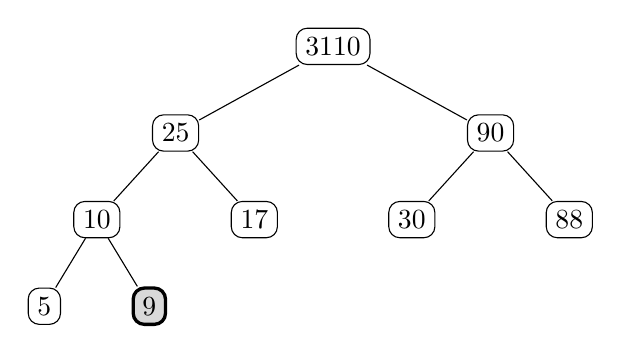
\begin{tikzpicture}[
  every node/.style = {tree node},
]
\node {3110}
  child { node {25}
    child { node {10}
      child { node {5} }
      child { node[very thick,fill=black!15!white] {9} }
    }
    child { node {17} }
  }
  child { node {90}
    child { node {30} }
    child { node {88} }
  }
;
\end{tikzpicture}
\end{center}
\caption{A binary heap. The last node is highlighted.}
\label{fig:heap}
\end{figure}

Given a binary heap, the operations of a priority queue can be
implemented as follows:
\begin{description}
\item{\textit{Insertion:}} To insert a value \code{x} into an empty
  heap, create a tree with \code{x} as the root and two empty
  children. To insert \code{x} into a non-empty heap \code{h} whose
  current root is \code{y}, recursively insert the smaller of \code{x}
  and \code{y} into the child of \code{h} that will contain the new
  last node.

  For example, when inserting the value $20$ into the heap in
  figure~\ref{fig:heap}, the new last node will be the left subchild
  of the node numbered $17$; so the smaller of $20$ and $3110$ (i.e.,
  $20$) is recursively inserted into the subtree with root $25$.

\item{\textit{Removal:}} By construction, the value that should be
  returned is always located at the root. However, removing the root
  produces two binary heaps. To merge these into a new binary heap,
  replace the root value with the value in the last node. If the
  resulting tree does not satisfy the heap property, then repair it by
  swapping the root value with the value stored at the root of the
  larger child, and recursively repair that subtree.

  For example, when removing the maximum element from the heap
  depicted in figure~\ref{fig:heap}, we begin by replacing the root
  ($3110$) with the last element ($9$). Then we swap the root ($9$)
  with the larger of its children ($90$). This causes the right
  subtree to violate the heap property, so we recursively repair the
  right subtree.
\end{description}

\newpage{}

\exercise{}
\label{ex:heappq}
[code] Implement the \code{PQueue.HeapImpl} module using a binary heap
as the data structure. Your implementation should match the
specification given in \filename{pQueue.mli}.

To help you, we have provided a function \code{path_to_last} that
computes the path from the root to the rightmost leaf of a complete
binary tree of a given size.\footnote{Astute observers will note that
  \code{path_to_last} is very similar to \code{int_to_bits} from
  problem set 2.} For example, the heap in Figure~\ref{fig:heap}
contains 9 nodes, and the last node can be reached from the root by
going left, then left, then right. Consequently \code{path_to_last 9}
returns \code{[Left; Left; Right]}. You may find this function helpful
for both insertion and removal: for the former you need to push the
inserted element towards the last node, while for the latter you need
to swap the root with the last node.

%% \exercise{} [written] Compare your implementation of priority queues
%% using binary heaps to the implementation using lists we have provided
%% in \code{PQueue.ListImpl}. Measure the performance of each
%% implementation by using the \code{PQueue.Heapsort} functor we have
%% provided to sort inputs ranging from small (fewer than 100 elements)
%% to large (up to 100,000 elements) in size. Briefly discuss the
%% situations under which you would prefer to use the list implementation
%% and when you would prefer the heap implementation. Consider
%% correctness, development time, and efficiency. The functions
%% \code{Util.time} and \code{Util.rand_list} may be useful.

\newpage{}
%%%%%%%%%%%%%%%%%%%%%%%%%%%%%%%%%%%%%%%%%%%%%%%%%%%%%%%%%%%%%%%%%%%%%%%%%%%%%%%%
\part{Puzzle Solver}
% \begin{comment}
% 	For this section of the problem set, we ask you to implement an $n\times n$
% 	grid puzzle, a generalization of the classic 15-puzzle, and a solver. The
% 	puzzle can be represented as a two-dimensional grid of height $n$ and width
% 	$n$, consisting of $n^2 - 1$ tiles and one gap; the tiles are numbered from 1
% 	to $n^2 - 1$, inclusive (see figure below).
% 
% 	$$\includegraphics[scale=.5]{puzzle.png}$$
% 
% 	Performing a move on this puzzle consists of sliding any tile adjacent to the
% 	gap into the gap. A ``solved'' puzzle is one where the tiles are arranged in
% 	increasing numerical order, starting from the top-left corner, going
% 	left-to-right and then top-to-bottom (\textbf{row-major order}), and
% 	positioning the gap at the bottom-right corner.
% 
% 	In the file $\tt{puzzle.ml}$, you will find an interface for a puzzle and a
% 	solver that takes in the puzzle and outputs a list of the moves (intermiediate
% 	puzzle configurations) whose last element is the solved puzzle (if one exists).
% \end{comment}
\begin{figure}
\centering
\begin{subfigure}{.5\textwidth}
  \centering
  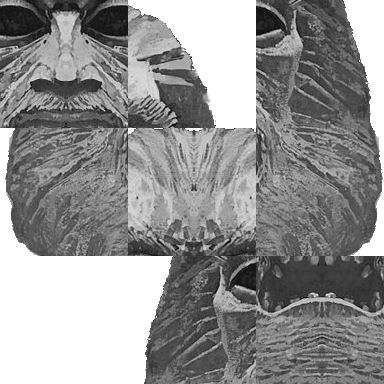
\includegraphics[scale=0.25]{images/tile.png}
  \caption{Sliding tile puzzle.}
  \label{fig:tile}
\end{subfigure}\begin{subfigure}{.5\textwidth}
  \centering
  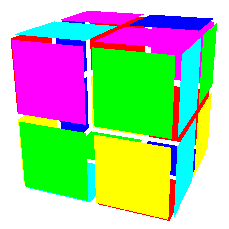
\includegraphics[scale=0.4]{images/cube.png}
  \caption{Rubik's cube.}
  \label{fig:rubik}
\end{subfigure}%
\caption{Two puzzle games.}
\label{fig:games}
\end{figure}

The goal of many puzzles is to find a sequence of moves that transform
an initial state into a final state. For example, in the sliding tile
puzzle (Figure~\ref{fig:tile}), the goal is to transform a scrambled
matrix of tiles into an unscrambled one by shifting tiles one at a
time, while in a Rubik's cube (Figure~\ref{fig:rubik}), the goal is to
transform a cube whose faces contain randomly colored squares into a
cube whose face contains squares of a single color using rotations.

Abstractly, these puzzles can be represented as (very large!) graphs
whose nodes correspond to configurations of the puzzle, and edges
correspond to feasible moves between states. A solution to the puzzle
is a path from the initial to final state in the
graph. Figure~\ref{fig:state-space} depicts a portion of the graph for
the sliding tile puzzle.

In this exercise you will implement a puzzle solver that searches for
a winning strategy in an arbitrary graph. Your solver will be generic
in the sense that it will work on the abstract representation of a
puzzle as a graph, so it will not need to know about the specific
details of the puzzle being solved. Hence, it will be possible to use
the same solver with sliding tile puzzles, Rubick's cubes, and others.

A simple way to search in a graph is to use depth-first or
breadth-first search. However, although these traversal strategies are
guaranteed to find a solution (if one exists), because the graphs
representing a puzzle tend to be very large, traversing the entire
graph is not feasible in general. A much better idea is to implement a
guided search strategy that explores the most promising paths
first. 

Such a search proceeds in the same manner as DFS or BFS: it maintains
a worklist of nodes to visit and a list of the nodes that have been
seen so far. At each step, it removes an element from the worklist and
processes it. However, unlike DFS (which removes the most recently
added node) or BFS (which removes the least recently added node),
guided search removes the most promising node. To break ties, if two
nodes are equally promising, it removes the node with the shorter
overall path from the initial node. This strategy is sometimes called
best-first search.

A good way to maintain the worklist for best-first search is to use a
priority queue ordered by goodness.  We recommend that you re-use
\code{PQueue.ListImpl} or \code{PQueue.HeapImpl} from the last
exercise.

\newpage{}

\exercise{} [code] Implement the \code{solve} function in the
\code{Solver.Make} functor (in the file \code{solver.ml}).  It takes a
puzzle state that has been instantiated in a non-goal state, and
outputs \code{Some l}, where \code{l} is a list of moves that solve
the puzzle, or \code{None} if no solution exists. Your solver should
make use of the types and functions in the \code{Solver.PUZZLE}
signature which define the graph representation of a puzzle, and the
heuristic function for determining whether a node is promising. See
the documentation provided in \filename{solver.mli} for further
details.

We have provided implementations of the sliding tile puzzle and the
Rubik's cube, along with graphical interfaces for visualizing games
being played. You can run them by running \filename{cubeMain.ml} and
\filename{tileMain.ml} respectively (using the \code{cs3110} tool!).
These programs generate a random puzzle, invoke your solver to solve
it, and then display an animation of the solution. To run the
animations, you must update the \code{cs3110} tool and install the SDL
graphics library. To do so, execute the following commands from the
command-line in the virtual machine:

\smallskip

\begin{ocaml}
% cd 3110-tools/cs3110-cli/student
% git pull
% make install
% sudo apt-get install libsdl1.2-dev libsdl-image1.2-dev libsdl-ttf2.0-dev
% opam install ocamlsdl
\end{ocaml}

\begin{figure}
\begin{center}
\begin{tikzpicture}[
  edge from parent path={
    (\tikzparentnode\tikzparentanchor) [->,decorate,decoration={bent,aspect=0.5}] -- (\tikzchildnode\tikzchildanchor)
    (\tikzchildnode\tikzchildanchor)   [->,decorate,decoration={bent,aspect=0.5}] -- (\tikzparentnode\tikzparentanchor)
  }
]

\tikzstyle{level 1}=[clockwise from=0, sibling angle=180, level distance=4cm]
\tikzstyle{level 2}=[clockwise from=40, sibling angle=80, level distance=3cm]
\tikzstyle{state}=[draw,rounded corners,thick,black]
\tikzstyle{move}=[above,sloped]
\tikzstyle{inv}=[below,sloped]


\newcommand{\pic}[2]{\includegraphics[width=#1]{images/tile#2.png}}

\node[state] (init) at ( 0, 0) {\pic{1.5cm}{}};
\node[state] (n)    at ( 0, 4) {\pic{1.5cm}{N}};
\node[state] (e)    at ( 4, 0) {\pic{1.5cm}{E}};
\node[state] (en)    at ( 4, 4) {\pic{1.5cm}{EN}};

%% \node[state] (ne)   at ( 5.5, 2) {\pic{.75cm}{NE}};
%% \node[state] (nn)   at ( 5.5,-2) {\pic{.75cm}{NN}};
%% \node[state] (e)    at (-3,-2) {\pic{.75cm}{E}};
%% \node[state] (en)   at (-3, 2) {\pic{.75cm}{EN}};

%% \node (ene) at (-5, 2) {$\cdots$};
%% \node (enw) at (-5, 1) {$\cdots$};
%% \node (enn) at (-5, 0) {$\cdots$};

%% \node (nen) at (7.5, 2) {$\cdots$};
%% \node (nes) at (7.5, 0) {$\cdots$};
%% \node (nne) at (7.5, -2) {$\cdots$};

\node[state] (sol) at (10, 0) {\pic{1.5cm}{sol}};

\node[above] at (0,-1.5) {\textit{initial state}};
\node[above] at (10,-1.5)  {\textit{final state}};

\tikzstyle{path}=[->,bend left=15, shorten >=1ex, shorten <=1ex,auto]
\tikzstyle{mycloud}=[draw,cloud,cloud puffs=9,minimum width=75pt,minimum height=50pt]
\node[mycloud] at (7, 0) { \large ? };
\node at (5.25, 0) { $\large \dots$};
\node at (8.75, 0) { $\large \dots$};
\draw[path] (init) edge node {N} (n);
\draw[path] (n) edge node {S} (init);
\draw[path] (init) edge node {E} (e);
\draw[path] (e) edge node {W} (init);
\draw[path] (e) edge node {N} (en);
\draw[path] (en) edge node {S} (e);
\draw[path] (en) edge node {W} (n);
\draw[path] (n) edge node {E} (en);


%%          edge node {E}  (e)
%%      (n) edge node {E} (ne)
%%          edge node {N} (nn)
%%          edge node {South} (init)
%%      (e) edge node {N} (en)
%%          edge node {W} (init)
%%     (ne) edge node {W} (n)
%%     (nn) edge node {S} (n)
%%     (en) edge node {S} (e)
%% ;

%% \path[path,ultra thin,bend left=0, gray]
%%   (en) edge (ene)
%%        edge (enw)
%%        edge (enn)
%%   (ne) edge (nee)
%%        edge (nen)
%%        edge (nes)
%%   (nn) edge (nne)
%% ;

%% \path[ultra thick,path]
%%   (init) edge (n)
%%   (n) edge (ne)
%%   [bend left=0]
%%   (ne) edge (nes)
%%   (nes) edge (sol);

\end{tikzpicture}
\end{center}
\caption{Partial graph for the sliding tile puzzle. The edges between
  nodes are labeled by the compass direction that the ``open'' tile
  needs to be shifted to move between the nodes.}
\label{fig:state-space}
\end{figure}

%%%%%%%%%%%%%%%%%%%%%%%%%%%%%%%%%%%%%%%%%%%%%%%%%%%%%%%%%%%%%%%%%%%%%%%%%%%%%%%%
% Part 3: Huffman Codes
%%%%%%%%%%%%%%%%%%%%%%%%%%%%%%%%%%%%%%%%%%%%%%%%%%%%%%%%%%%%%%%%%%%%%%%%%%%%%%%%
\newpage{}

\part{Huffman Coding}

Huffman coding is a data compression technique that analyzes the
frequencies of bytes occuring in a string. Characters that occur
frequently are encoded using shorter bitstrings, while those that
occur infrequently are encoded using longer bitstrings.

\begin{figure}
\hfill
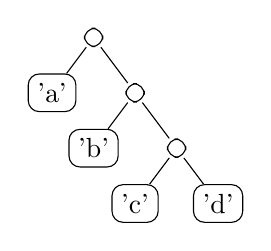
\begin{tikzpicture}[
  baseline,
  level/.style = {sibling distance=3em, level distance=2em},
  every node/.style = {tree node},
%  level 1/.style = {sibling distance=6em, level distance=.5cm},
%  level 2/.style = {sibling distance=6em, level distance=1cm},
%  level 3/.style = {sibling distance=3em, level distance=1cm}
]

\node {}
  child { node {\code{'a'}} }
  child { node {}
    child { node {\code{'b'}} }
    child { node {}
      child { node {\code{'c'}} }
      child { node {\code{'d'}} }
    }
  }
;
\end{tikzpicture}
\hfill
\begin{tabular}[t]{ll}
Character & Encoding \\ \hline
'a' & 0 \\
'b' & 10 \\
'c' & 110 \\
'd' & 111 \\
\end{tabular}
\hfill{}

\caption{A Huffman tree and the corresponding encoding}
\label{fig:hufftree}
\end{figure}

A huffman encoding can be represented as a binary tree, often called a
\emph{Huffman tree}, with characters at the leaves. The encoding of a
given character is given by the path from the root to that character:
each left branch adds a $0$ bit to the bitstring and each right branch
adds a $1$ bit. Figure~\ref{fig:hufftree} depicts a Huffman tree and
the corresponding encoding of a single character.

Huffman tree encodings have the property that a bit sequence formed by
concatenating the encodings of letters can be uniquely decoded. For
example, using the encoding represented by figure~\ref{fig:hufftree},
the bit string \code{1100111010100} is decoded as \code{"cadabba"}.

If the frequencies of the characters in a file are known, an optimal
Huffman tree can be built using a simple greedy algorithm that
maintains a priority queue of partial Huffman trees. Initially the
queue contains a leaf for each character, with its priority given by
the frequency of that character in the original string. Then, at each
step, we remove the two trees with the lowest frequencies, and combine
them into a single tree. This tree is then reinserted into the queue
with priority given by the sum of their frequencies. This process is
repeated until only a single tree remains; this tree is the optimal
Huffman tree for the given input frequencies. For example, the tree in
figure~\ref{fig:hufftree} can be built from the string
\code{"cadabba"} using the following sequence of steps:

\bigskip

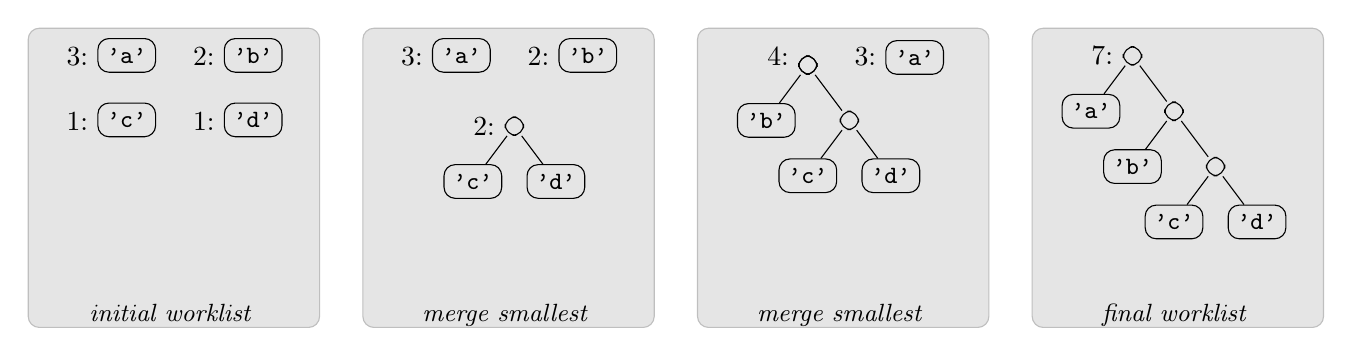
\begin{tikzpicture}[
  level/.style = {sibling distance=3em, level distance=2em},
  worklist label/.style = {font={\small\it}, anchor=base, yshift=.5ex},
  worklist/.style = {draw=black!25!white, fill=black!10!white, rounded corners},
  label/.style = {},
  tree/.style = {tree node,every node/.style = {tree node}, font={\tt \small}},
]

\newcommand{\worklist}[1]{
  \draw[worklist] (-1.8, 0) rectangle (1.9,-3.8);
  \node[worklist label] at (0, -3.8) {#1};
}

\begin{scope}
\worklist{initial worklist}

\matrix[row sep=1em,anchor=north] {
  \node[label] {3:}; & \node[tree] {'a'}; &[1em]
  \node[label] {2:}; & \node[tree] {'b'}; \\
  \node[label] {1:}; & \node[tree] {'c'}; &
  \node[label] {1:}; & \node[tree] {'d'}; \\
};
\end{scope}

\begin{scope}[xshift=4.25cm]
\worklist{merge smallest};

\matrix[anchor=north] (top) {
  \node[label]{3:}; & \node[tree] {'a'}; &[1em]
  \node[label]{2:}; & \node[tree] {'b'}; \\
};

\coordinate (root) at ($(top.south)-(0,1.5em)$);
\node[label,left] at (root) {2:};
\path (root) [tree] node[right] {}
  child { node {\code{'c'}} }
  child { node {\code{'d'}} }
;
\end{scope}

\begin{scope}[xshift=8.5cm]
\worklist{merge smallest};

\matrix[anchor=north, nodes={anchor=base}] at (0.15,0) {
  \node[label] {4:}; & \node[tree] (root) {}; &[1em]
  \node[label] {3:}; & \node[tree] {'a'}; \\
};

\path (root) [tree] node {}
  child { node {\code{'b'}} }
  child { node {}
    child { node {\code{'c'}} }
    child { node {\code{'d'}} }
  }
;
\end{scope}

\begin{scope}[xshift=12.75cm]
\worklist{final worklist};

\coordinate (root) at (-.65cm,-1em);
\node [left] at (root) {7:};
\path [tree] (root) node [right] {}
  child { node {\code{'a'}} }
  child { node {}
    child { node {\code{'b'}} }
    child { node {}
      child { node {\code{'c'}} }
      child { node {\code{'d'}} }
    }
  }
;
\end{scope}

\end{tikzpicture}

% [a, 3; b, 2; c, 1; d, 1]
% 
% [a, 3; b, 2; cd, 2]
% 
% [a, 3; bcd, 4]
% 
% [abcd, 7]

\newpage{}

\exercise{} 

[code] In the file \filename{huffman.ml}, implement the
\code{build_tree} function to construct a Huffman tree from the
provided character list.  If the input list is empty, the
\code{build_tree} function should return \code{Empty}. It should use
one of the implementations of priority queues: either
\code{PQueue.ListImpl} or \code{PQueue.HeapImpl}.\footnote{Note that
  because the remove operation returns the greatest element, you will
  have to invert the usual ordering on integers so that smaller
  frequences rank higher.}

%% JNF: what is written document? There's no question here. And this
%% is really open-ended. Let's cut it.
%
%% In your written document,
%% briefly discuss which \code{PQ} implementation you used and why.
\exercise{} 

[code] Implement the \code{encode} and \code{decode} functions in
\filename{huffman.ml}.  These functions are specified in detail in
\filename{huffman.mli}. We have provided you with driver programs
\filename{compress.ml} and \filename{decompress.ml} that compress and
decompress whole files. You can test your implementation by running
these commands using \filename{cs3110} tool. For example:
\begin{ocaml}
> cs3110 compile compress.ml
> cs3110 compile decompress.ml
> cs3110 run compress.ml ../data/Conrad.txt > Conrad.huff
> du -b ../data/Conrad.txt
213304	
> du -b Conrad.huff
118727
> cs3110 run decompress.ml Conrad.huff > Conrad.out
> diff -s ../data/Conrad.txt Conrad.out
Files ../data/Conrad.txt and Conrad.out are identical
\end{ocaml}

This example shows that the compressed file is about 55\% of the size of
the original.  This is a typical savings for Huffman coding on large files;
smaller files typically get less benefit from compression because there is less
diversity in character frequency and because the Huffman tree itself must also
be stored in the file.  The \filename{data/} directory contains a number of
compressed and uncompressed files that you can use to test your implementation.

\newpage{}

\part{Formal Reasoning}

In this part of the assignment, you will investigate proofs of program
equivalence using structural induction and the substitution
model. Your solutions to these exercises should be submitted in a
single file \code{reasoning.pdf} that can be created using any
software you like.

\exercise{} 
[written] Recall the binary tree data type:
\begin{ocaml}
type 'a bintree = 
    Leaf 
  | Node of 'a bintree * 'a * 'a bintree
\end{ocaml}
Let $P(t)$ be an arbitrary predicate on binary trees. State the
structural induction principle for the \code{'a bintree} datatype as a
logical formula of the form ``\( \left(~\dots~\right) \Longrightarrow
\forall t.\, P(t) \).''

\exercise{} 
[written] 
Consider the following recursive function, 
\begin{ocaml}
let rec tree_sum = 
  (fun t -> 
    match t with 
     | Leaf -> 0 
     | Node(l,x,r) -> x + (tree_sum l) + (tree_sum r)) in 
tree_sum t
\end{ocaml}
and an equivalent function written using \code{tree_fold}:
\begin{ocaml}
let rec tree_fold = 
  (fun a -> fun f -> fun t -> 
    match t with 
     | Leaf -> a 
     | Node(l,x,r) -> f x (tree_fold a f l) (tree_fold a f r)) in 
tree_fold 0 (fun x l r -> x + l + r) t
\end{ocaml}
Assume that we have already generated fresh variables \code{tree_sum'}
and \code{tree_fold'}, and added new reduction rules to handle the
recursive definitions:
%
\begin{alltt}
tree_fold' \(\longrightarrow\) (fun a -> fun f -> fun t ->
\qquad\qquad\qquad\qquad match t with
\qquad\qquad\qquad\qquad\quad   | Leaf -> a
\qquad\qquad\qquad\qquad\quad   | Node(l,x,r) -> f x (tree_fold' a f l) (tree_fold' a f r))

tree_sum' \(\longrightarrow\) (fun t ->
\qquad\qquad\qquad\qquad match t with
\qquad\qquad\qquad\qquad\quad | Leaf -> 0
\qquad\qquad\qquad\qquad\quad | Node(l,x,r) -> x + (tree_sum' l) + (tree_sum' r))
\end{alltt}
%
Give a careful proof of the following
equivalence:
\[
\begin{array}{l}
\text{\code{let tree_fold = tree_fold' in tree_fold 0 (fun x l r -> x + l + r) t}} = \\
\text{\code{let tree_sum = tree_sum' in tree_sum t}}
\end{array}
\]
You should show that both sides of the equality reduce to the same
value in the substitution model. To complete the proof, you will
likely need to prove a lemma $\forall t.\,P(t)$, where $P(t)$ is the
predicate:
\[
\begin{array}{ll}
P(t) \triangleq 
& \text{\code{(fun a -> fun f -> fun t ->}}\\
& \qquad\text{\code{match t with}}\\
& \qquad\quad\text{\code{ | Leaf -> a}}\\
& \qquad\quad\text{\code{ | Node(l,x,r) -> f x (tree\_fold' a f l) (tree\_fold' a f r))}}\\
& \text{\code{0 (fun x l r -> x + l + r) t}}\\
& = \\
& \text{\code{(fun t ->}}\\
& \qquad\text{\code{match t with}}\\
& \qquad\quad\text{\code{ | Leaf -> 0}}\\
& \qquad\quad\text{\code{| Node(l,x,r) -> x + (tree\_sum' l) + (tree\_sum' r))}}\\
& \text{\code{t}}\\
\end{array}
\]
Your proof of this lemma should use the structural induction principle
on binary trees.

\newpage{}

\setlength{\parskip}{0.1em}
\section*{Getting Started}

Because this is a larger assignment, we have provided you with a lot of
code to get started. 

\begin{itemize}
\item \filename{writeup/} this writeup.
\item \filename{doc/} automatically generated ocamldoc documentation
  for the starter code provided in \filename{release}.
\item \filename{data/} data files for testing your Huffman implementation
\item \filename{release/} \begin{itemize}
  \item \filename{huffman.\{ml,mli\}}, \filename{pQueue.\{ml,mli\}},
        \filename{solver.\{ml,mli\}} modules to implement.
  \item \filename{animation.\{ml,mli\}},
    \filename{tilePuzzle.\{ml,mli\}},
    \filename{cubePuzzle.\{ml,mli\}}, \filename{zardoz.png} support
    files for the animations for the puzzle solver.
  \item \filename{compress.ml}, \filename{decompress.ml},
    \filename{tileMain.ml} \filename{cubeMain.ml} driver programs for
    testing your Huffman and solver implementations.
  \item \filename{util.\{ml,mli\}} utility functions  you may find useful.
  \end{itemize}
\end{itemize}

\section*{Comments}

We would like to know how this assignment went for you.  Were there
any parts that you didn't finish or wish you had done in a better way?
Which parts were particularly fun or interesting?  Did you do any
Karma problems?

\section*{Karma suggestions}

\begin{itemize}
\item Implement more puzzles for your solver.  If you're feeling
  adventurous, add animations!

\item For the Rubik's cube puzzle, we intentionally generated inputs
  with short solutions (fewer than 8 moves) because the search space
  grows exponentially. Similarly, we only generate 8-tile puzzles.
  Performance can be improved, by using better heuristics, algorithms,
  or data structures.  Implement a solver that is efficient enough to
  handle much larger instances of the puzzles.

\item See what impact the OCaml native code compiler \code{ocamlopt}
  has on the performance of your priority queue implementations. 

\item The Wikipedia entry on Huffman coding contains a wealth of
  variations on Huffman encoding.  Find one that interests you and
  implement it.

\item We did not specify how to break ties when selecting trees in the
  \code{build_tree} function, so there are multiple valid
  implementations.  Determine whether different choices can produce
  encodings with a different length.
\end{itemize}

\end{document}
